\documentclass[a4paper]{article}

\usepackage[utf8x]{inputenc}    
\usepackage[T1]{fontenc}
\usepackage[spanish]{babel}
\usepackage{multicol}

\usepackage{wrapfig}
\usepackage{graphicx}

\usepackage{bm}
\usepackage{amsxtra} 
\usepackage{amssymb}% to get the \mathbb alphabet
\usepackage{amsmath}

\usepackage[box,completemulti,separateanswersheet]{automultiplechoice}    
\def\AMCformQuestion#1{\vspace{\AMCformVSpace}\par {\sc Pregunta #1:} }    
\def\AMCbeginQuestion#1#2{\par\noindent{\bf Pregunta #1}#2\hspace*{1em}}
\def\AMCcleardoublepage{\ifodd\thepage\clearpage\mbox{}\fi\clearpage}

\begin{document}

\AMCrandomseed{1237893}

%%%%%%%%%%%%%%%%%%%%%%%%%%%%%%%%%%%%%%%%%%%%%%%%%%%%%%%%%%%%%%%%%%%%%%%%%%%%%
\element{test1}{
\begin{question}{p1}
El valor del desplazamiento en direcci\'on $x$ del nodo $A$,
calculado con integración reducida, vale aproximadamente:\begin{multicols}{2}
\begin{choices}
	\correctchoice{$-34.8$ mm}
	\wrongchoice{$-12.3$ mm}
	\wrongchoice{$3.4$ mm}
	\wrongchoice{$-21.8$ mm}
\end{choices}
\end{multicols}
\end{question}
}
%%%%%%%%%%%%%%%%%%%%%%%%%%%%%%%%%%%%%%%%%%%%%%%%%%%%%%%%%%%%%%%%%%%%%%%%%%%%%
\element{test1}{
\begin{question}{p2}
El valor del desplazamiento en direcci\'on $y$ del nodo $B$, calculado con elementos mixtos, vale aproximadamente:
\begin{multicols}{2}
\begin{choices}
	\correctchoice{$15.0$ mm}
	\wrongchoice{$-34.1$ mm}
	\wrongchoice{$0.87$ mm}
	\wrongchoice{$9.21$ mm}
\end{choices}
\end{multicols}
\end{question}
}
%%%%%%%%%%%%%%%%%%%%%%%%%%%%%%%%%%%%%%%%%%%%%%%%%%%%%%%%%%%%%%%%%%%%%%%%%%%%%
\element{test1}{
\begin{question}{p3}
El valor del desplazamiento en direcci\'on $y$ del nodo $B$, calculado con elementos con modos incompatibles, vale aproximadamente:
\begin{multicols}{2}
\begin{choices}
	\correctchoice{$21.5$ mm}
	\wrongchoice{$ -12.1$ mm}
	\wrongchoice{$ 35.8$ mm}
	\wrongchoice{$ 0.67$ mm}
\end{choices}
\end{multicols}
\end{question}
}
%%%%%%%%%%%%%%%%%%%%%%%%%%%%%%%%%%%%%%%%%%%%%%%%%%%%%%%%%%%%%%%%%%%%%%%%%%%%%
\element{test1}{
\begin{question}{p4}
	Para el cálculo con integración reducida, el valor m\'aximo de la tensi\'on de \emph{von Mises} es aproximadamente:
\begin{multicols}{2}
\begin{choices}
	\correctchoice{$27$ MPa}
	\wrongchoice{$ 12$ MPa}
	\wrongchoice{$ 53$ MPa}
	\wrongchoice{$ 6$ MPa}
\end{choices}
\end{multicols}
\end{question}
}
%%%%%%%%%%%%%%%%%%%%%%%%%%%%%%%%%%%%%%%%%%%%%%%%%%%%%%%%%%%%%%%%%%%%%%%%%%%%%
\element{test1}{
\begin{question}{p5}
	Para el cálculo con elementos mixtos, el valor m\'aximo de tracción, $\sigma_1$ es aproximadamente:
\begin{multicols}{2}
\begin{choices}
	\correctchoice{$ 36$ MPa}
	\wrongchoice{$  21$ MPa}
	\wrongchoice{$  12$ MPa}
	\wrongchoice{$  9$ MPa}
\end{choices}
\end{multicols}
\end{question}
}
%%%%%%%%%%%%%%%%%%%%%%%%%%%%%%%%%%%%%%%%%%%%%%%%%%%%%%%%%%%%%%%%%%%%%%%%%%%%%
\element{test1}{
\begin{question}{p6}
	Para el cálculo con modos incompatibles, el valor m\'aximo de compresión en valor absoluto, observado en $\sigma_3$ es aproximadamente:
\begin{multicols}{2}
\begin{choices}
	\correctchoice{$ 47$ MPa}
	\wrongchoice{$  31$ MPa}
	\wrongchoice{$ 1 $ MPa}
	\wrongchoice{$ 7 $ MPa}
\end{choices}
\end{multicols}
\end{question}
}
%%%%%%%%%%%%%%%%%%%%%%%%%%%%%%%%%%%%%%%%%%%%%%%%%%%%%%%%%%%%%%%%%%%%%%%%%%%%% 
\element{test1}{
\begin{question}{p7}
De acuerdo con los valores de los contornos de la tensi\'on de
\emph{von Mises}, la posible zona de rotura del perfil es:
\begin{multicols}{2}
\begin{choices}
	\correctchoice{Con los tres modelos, en los puntos en que se aplican las cargas}
	\wrongchoice{Con el modelo de modos incompatibles, en los puntos en que se aplican las cargas. Con los modelos de elementos mixtos e integración reducida, en la zona central de la cara interna}
	\wrongchoice{Con los modelos de elementos mixtos e integración reducida,
en los puntos en que se aplican las cargas. Con el modelo de modos incompatibles, en la zona central de la cara interna}
	\wrongchoice{Con los tres modelos, en la zona central de la cara
interna}
\end{choices}
\end{multicols}
\end{question}
}
%%%%%%%%%%%%%%%%%%%%%%%%%%%%%%%%%%%%%%%%%%%%%%%%%%%%%%%%%%%%%%%%%%%%%%%%%%%%%
\element{test1}{
\begin{question}{p8}
El valor de $\sigma_{yy}$ en el centroide delemento más cercano al punto $B$,
	calculado con elementos mixtos, vale aproximadamente:
\begin{multicols}{2}
\begin{choices}
       \correctchoice{$10.3$ MPa}
        \wrongchoice{$14.1$ MPa}
        \wrongchoice{$9.3$ MPa}
        \wrongchoice{$41.0$ MPa}
\end{choices}
\end{multicols}
\end{question}
}
%%%%%%%%%%%%%%%%%%%%%%%%%%%%%%%%%%%%%%%%%%%%%%%%%%%%%%%%%%%%%%%%%%%%%%%%%%%%%
\element{test1}{
\begin{question}{p9}
El fenómeno del ``hourglassing'':
\begin{multicols}{2}
	\begin{choices}
		\correctchoice{Puede aparecer cuando las matrices de rigidez
			se calculan con una regla de integración reducida}
		\wrongchoice{Consiste en el cambio del signo de la presión en elementos
			adyacentes, denominándose también problema del ``tablero de damas'' o 
			``checkerboard''}
		\wrongchoice{Puede aparecer en problemas de incompresibilidad,
			con independecia del orden que tenga la regla de integración (o cuadratura)
			empleada}
		\wrongchoice{Sólo aparece en elementos con funciones de forma cuadráticas}
	\end{choices}
\end{multicols}
\end{question}
}
%%%%%%%%%%%%%%%%%%%%%%%%%%%%%%%%%%%%%%%%%%%%%%%%%%%%%%%%%%%%%%%%%%%%%%%%%%%%%
\element{test1}{
\begin{question}{p10}
La formulación $\overline{\bm{B}}$ de elementos finitos:
\begin{multicols}{2}
	\begin{choices}
		\correctchoice{Se basa en modificar la matriz de interpolación de
			deformaciones estándar}
		\wrongchoice{Se basa en remplazar la matriz de interpolación de
			deformaciones por un vector de deformaciones libre de bloqueo}
		\wrongchoice{Se basa en considerar como variable básica la presión adicionalmente a los desplazamientos nodales}
		\wrongchoice{Los elementos con esta formulación no pasan la prueba de la parcela}
	\end{choices}
\end{multicols}
\end{question}
}
%%%%%%%%%%%%%%%%%%%%%%%%%%%%%%%%%%%%%%%%%%%%%

\scoringDefaultS{b=1,m=-1/(N-1)}

\onecopy{30}{    

%%% beginning of the test sheet header:    

\noindent{\large\bf Método de los Elementos Finitos  \hfill MUECYM \hfill TEST \# 4}
\begin{center}
%\vspace*{.1cm}
%Se atribuirá puntuación negativa a las respuestas incorrectas.\\
\vspace*{.1cm}
10 dic 2024. \hspace{7cm} Tiempo: 60 minutos.\\


\end{center}

\vspace{1ex}

La estructura de la figura, cuyas dimensiones están indicadas en la misma,
está fabricada con un material cuyas propiedades mecánicas son
$E=20.5$ GPa y $\nu=0.23$. Las cargas aplicadas tienen todas el mismo
valor $F=1000$ kN. Las condiciones de contorno a aplicar son las
correspondientes a que los planos $OXY$, $OXZ$ y $OYZ$ sean planos de
simetría.

La discretización a considerar son $2$ elementos en el espesor y $16 \times 16$
elementos en las caras verticales (situadas fuera de los planos
coordenados). Para resolver el problema se utilizarán elementos lineales hexaédricos
de $8$ nodos con las diferentes formulaciones que si indican a continuación: integración reducida, formulación mixta y modos incompatibles.


\vspace{5mm}
\begin{center}
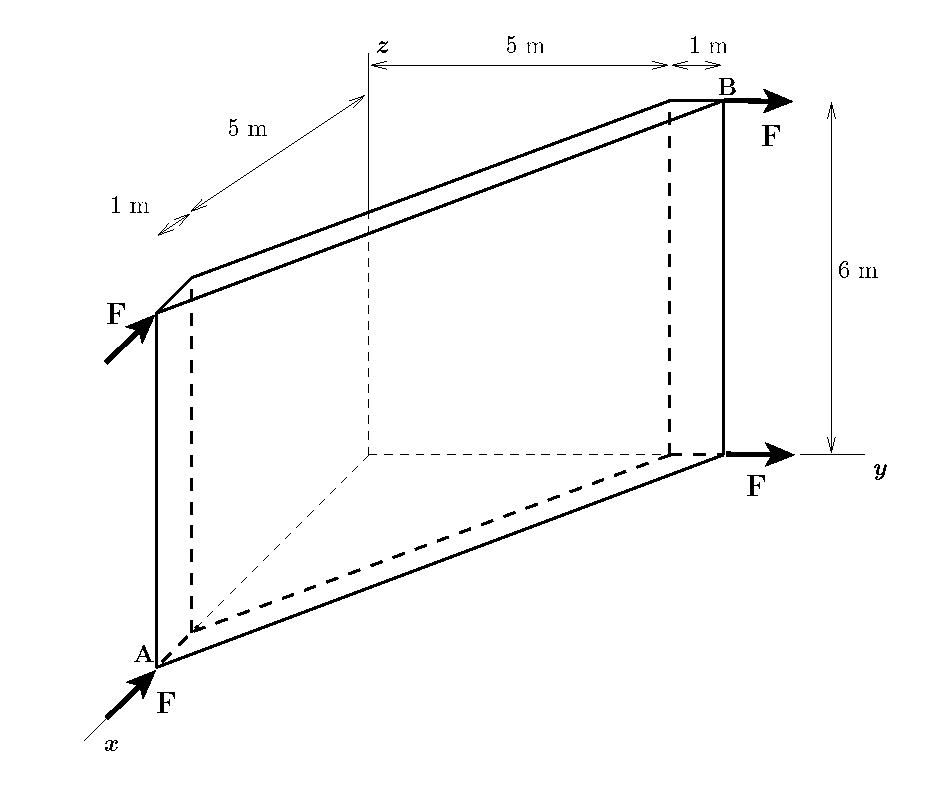
\includegraphics[width=0.8\textwidth]{ejerc4}
\end{center}

\hrulefill
\vspace{4mm}

%%% end of the header

\shufflegroup{test1}
\insertgroup{test1}

%\AMCcleardoublepage    
\clearpage

\AMCformBegin    

%%% beginning of the answer sheet header

\noindent\AMCcode{nummat}{2}\hspace*{\fill}
\begin{minipage}{.7\linewidth}
$\longleftarrow{}$ Escriba su número de matrícula marcando los dígitos
en los recuadros (con ceros a la izquierda si el número es de menos de dos dígitos) y el nombre y apellidos debajo.

\vspace{3ex}

\namefield{\fbox{
   \begin{minipage}{.9\linewidth}
     Apellidos, Nombre:

     \vspace*{.5cm}\dotfill
     \vspace*{1mm}
   \end{minipage}
 }}
\end{minipage}

\begin{center}
 \bf\em Debe dar las respuestas exclusivamente en esta hoja (las respuestas en las demás hojas no serán tenidas en cuenta).
\end{center}

%%% end of the answer sheet header


\AMCform    

\AMCcleardoublepage    

}  

\end{document}
